% Created by tikzDevice version 0.10.1 on 2018-01-15 21:00:14
% !TEX encoding = UTF-8 Unicode
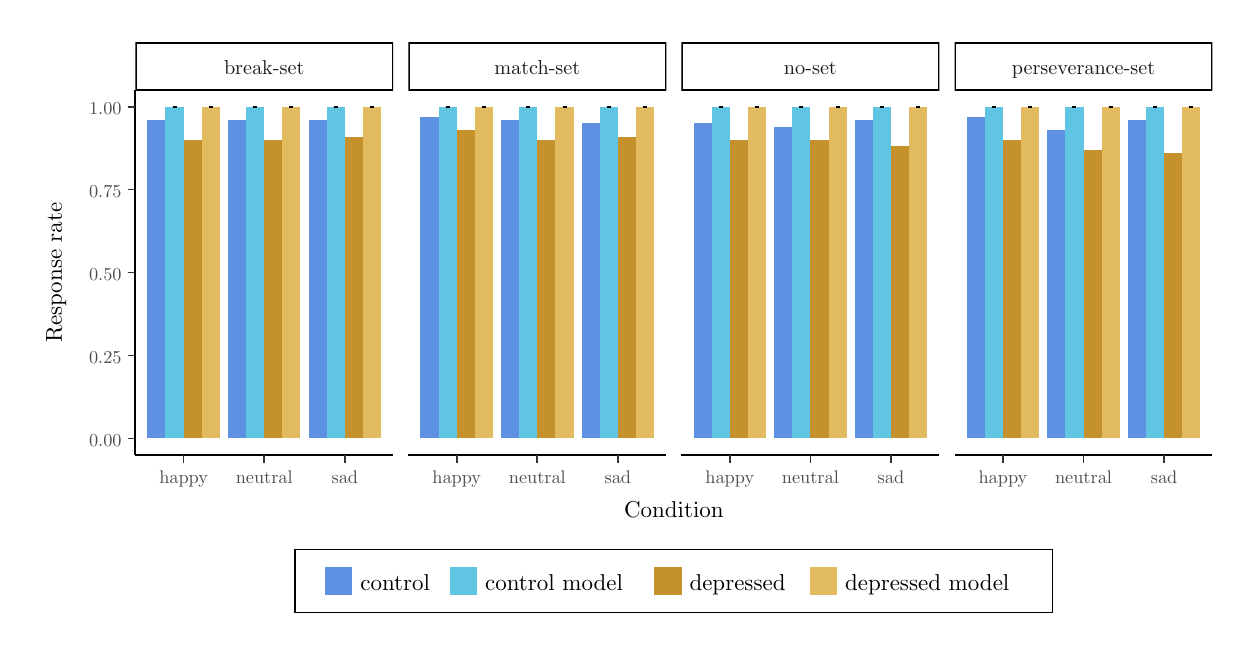
\begin{tikzpicture}[x=1pt,y=1pt]
\definecolor{fillColor}{RGB}{255,255,255}
\path[use as bounding box,fill=fillColor,fill opacity=0.00] (0,0) rectangle (433.62,216.81);
\begin{scope}
\path[clip] (  0.00,  0.00) rectangle (433.62,216.81);
\definecolor{drawColor}{RGB}{255,255,255}
\definecolor{fillColor}{RGB}{255,255,255}

\path[draw=drawColor,line width= 0.6pt,line join=round,line cap=round,fill=fillColor] (  0.00,  0.00) rectangle (433.62,216.81);
\end{scope}
\begin{scope}
\path[clip] ( 38.88, 62.37) rectangle (132.07,194.25);
\definecolor{fillColor}{RGB}{255,255,255}

\path[fill=fillColor] ( 38.88, 62.37) rectangle (132.07,194.25);
\definecolor{fillColor}{RGB}{226,186,95}

\path[fill=fillColor] ( 62.91, 68.36) rectangle ( 69.46,188.25);
\definecolor{fillColor}{RGB}{196,145,45}

\path[fill=fillColor] ( 56.36, 68.36) rectangle ( 62.91,176.27);
\definecolor{fillColor}{RGB}{95,197,226}

\path[fill=fillColor] ( 49.80, 68.36) rectangle ( 56.36,188.25);
\definecolor{fillColor}{RGB}{95,145,226}

\path[fill=fillColor] ( 43.25, 68.36) rectangle ( 49.80,183.46);
\definecolor{fillColor}{RGB}{226,186,95}

\path[fill=fillColor] ( 92.03, 68.36) rectangle ( 98.58,188.25);
\definecolor{fillColor}{RGB}{196,145,45}

\path[fill=fillColor] ( 85.48, 68.36) rectangle ( 92.03,176.27);
\definecolor{fillColor}{RGB}{95,197,226}

\path[fill=fillColor] ( 78.92, 68.36) rectangle ( 85.48,188.25);
\definecolor{fillColor}{RGB}{95,145,226}

\path[fill=fillColor] ( 72.37, 68.36) rectangle ( 78.92,183.46);
\definecolor{fillColor}{RGB}{226,186,95}

\path[fill=fillColor] (121.15, 68.36) rectangle (127.70,188.25);
\definecolor{fillColor}{RGB}{196,145,45}

\path[fill=fillColor] (114.60, 68.36) rectangle (121.15,177.46);
\definecolor{fillColor}{RGB}{95,197,226}

\path[fill=fillColor] (108.04, 68.36) rectangle (114.60,188.25);
\definecolor{fillColor}{RGB}{95,145,226}

\path[fill=fillColor] (101.49, 68.36) rectangle (108.04,183.46);
\definecolor{drawColor}{RGB}{0,0,0}

\path[draw=drawColor,line width= 0.6pt,line join=round] ( 65.46,188.25) --
	( 66.91,188.25);

\path[draw=drawColor,line width= 0.6pt,line join=round] ( 66.18,188.25) --
	( 66.18,188.25);

\path[draw=drawColor,line width= 0.6pt,line join=round] ( 65.46,188.25) --
	( 66.91,188.25);

\path[draw=drawColor,line width= 0.6pt,line join=round] ( 52.35,188.25) --
	( 53.81,188.25);

\path[draw=drawColor,line width= 0.6pt,line join=round] ( 53.08,188.25) --
	( 53.08,188.25);

\path[draw=drawColor,line width= 0.6pt,line join=round] ( 52.35,188.25) --
	( 53.81,188.25);

\path[draw=drawColor,line width= 0.6pt,line join=round] ( 94.58,188.25) --
	( 96.03,188.25);

\path[draw=drawColor,line width= 0.6pt,line join=round] ( 95.30,188.25) --
	( 95.30,188.25);

\path[draw=drawColor,line width= 0.6pt,line join=round] ( 94.58,188.25) --
	( 96.03,188.25);

\path[draw=drawColor,line width= 0.6pt,line join=round] ( 81.47,188.25) --
	( 82.93,188.25);

\path[draw=drawColor,line width= 0.6pt,line join=round] ( 82.20,188.25) --
	( 82.20,188.25);

\path[draw=drawColor,line width= 0.6pt,line join=round] ( 81.47,188.25) --
	( 82.93,188.25);

\path[draw=drawColor,line width= 0.6pt,line join=round] (123.70,188.25) --
	(125.15,188.25);

\path[draw=drawColor,line width= 0.6pt,line join=round] (124.42,188.25) --
	(124.42,188.25);

\path[draw=drawColor,line width= 0.6pt,line join=round] (123.70,188.25) --
	(125.15,188.25);

\path[draw=drawColor,line width= 0.6pt,line join=round] (110.59,188.25) --
	(112.05,188.25);

\path[draw=drawColor,line width= 0.6pt,line join=round] (111.32,188.25) --
	(111.32,188.25);

\path[draw=drawColor,line width= 0.6pt,line join=round] (110.59,188.25) --
	(112.05,188.25);
\end{scope}
\begin{scope}
\path[clip] (137.57, 62.37) rectangle (230.75,194.25);
\definecolor{fillColor}{RGB}{255,255,255}

\path[fill=fillColor] (137.57, 62.37) rectangle (230.75,194.25);
\definecolor{fillColor}{RGB}{226,186,95}

\path[fill=fillColor] (161.59, 68.36) rectangle (168.14,188.25);
\definecolor{fillColor}{RGB}{196,145,45}

\path[fill=fillColor] (155.04, 68.36) rectangle (161.59,179.86);
\definecolor{fillColor}{RGB}{95,197,226}

\path[fill=fillColor] (148.49, 68.36) rectangle (155.04,188.25);
\definecolor{fillColor}{RGB}{95,145,226}

\path[fill=fillColor] (141.94, 68.36) rectangle (148.49,184.66);
\definecolor{fillColor}{RGB}{226,186,95}

\path[fill=fillColor] (190.71, 68.36) rectangle (197.26,188.25);
\definecolor{fillColor}{RGB}{196,145,45}

\path[fill=fillColor] (184.16, 68.36) rectangle (190.71,176.27);
\definecolor{fillColor}{RGB}{95,197,226}

\path[fill=fillColor] (177.61, 68.36) rectangle (184.16,188.25);
\definecolor{fillColor}{RGB}{95,145,226}

\path[fill=fillColor] (171.06, 68.36) rectangle (177.61,183.46);
\definecolor{fillColor}{RGB}{226,186,95}

\path[fill=fillColor] (219.83, 68.36) rectangle (226.38,188.25);
\definecolor{fillColor}{RGB}{196,145,45}

\path[fill=fillColor] (213.28, 68.36) rectangle (219.83,177.46);
\definecolor{fillColor}{RGB}{95,197,226}

\path[fill=fillColor] (206.73, 68.36) rectangle (213.28,188.25);
\definecolor{fillColor}{RGB}{95,145,226}

\path[fill=fillColor] (200.18, 68.36) rectangle (206.73,182.26);
\definecolor{drawColor}{RGB}{0,0,0}

\path[draw=drawColor,line width= 0.6pt,line join=round] (164.14,188.25) --
	(165.60,188.25);

\path[draw=drawColor,line width= 0.6pt,line join=round] (164.87,188.25) --
	(164.87,188.25);

\path[draw=drawColor,line width= 0.6pt,line join=round] (164.14,188.25) --
	(165.60,188.25);

\path[draw=drawColor,line width= 0.6pt,line join=round] (151.04,188.25) --
	(152.49,188.25);

\path[draw=drawColor,line width= 0.6pt,line join=round] (151.76,188.25) --
	(151.76,188.25);

\path[draw=drawColor,line width= 0.6pt,line join=round] (151.04,188.25) --
	(152.49,188.25);

\path[draw=drawColor,line width= 0.6pt,line join=round] (193.26,188.25) --
	(194.72,188.25);

\path[draw=drawColor,line width= 0.6pt,line join=round] (193.99,188.25) --
	(193.99,188.25);

\path[draw=drawColor,line width= 0.6pt,line join=round] (193.26,188.25) --
	(194.72,188.25);

\path[draw=drawColor,line width= 0.6pt,line join=round] (180.16,188.25) --
	(181.61,188.25);

\path[draw=drawColor,line width= 0.6pt,line join=round] (180.88,188.25) --
	(180.88,188.25);

\path[draw=drawColor,line width= 0.6pt,line join=round] (180.16,188.25) --
	(181.61,188.25);

\path[draw=drawColor,line width= 0.6pt,line join=round] (222.38,188.25) --
	(223.84,188.25);

\path[draw=drawColor,line width= 0.6pt,line join=round] (223.11,188.25) --
	(223.11,188.25);

\path[draw=drawColor,line width= 0.6pt,line join=round] (222.38,188.25) --
	(223.84,188.25);

\path[draw=drawColor,line width= 0.6pt,line join=round] (209.28,188.25) --
	(210.73,188.25);

\path[draw=drawColor,line width= 0.6pt,line join=round] (210.00,188.25) --
	(210.00,188.25);

\path[draw=drawColor,line width= 0.6pt,line join=round] (209.28,188.25) --
	(210.73,188.25);
\end{scope}
\begin{scope}
\path[clip] (236.25, 62.37) rectangle (329.44,194.25);
\definecolor{fillColor}{RGB}{255,255,255}

\path[fill=fillColor] (236.25, 62.37) rectangle (329.44,194.25);
\definecolor{fillColor}{RGB}{226,186,95}

\path[fill=fillColor] (260.28, 68.36) rectangle (266.83,188.25);
\definecolor{fillColor}{RGB}{196,145,45}

\path[fill=fillColor] (253.72, 68.36) rectangle (260.28,176.27);
\definecolor{fillColor}{RGB}{95,197,226}

\path[fill=fillColor] (247.17, 68.36) rectangle (253.72,188.25);
\definecolor{fillColor}{RGB}{95,145,226}

\path[fill=fillColor] (240.62, 68.36) rectangle (247.17,182.26);
\definecolor{fillColor}{RGB}{226,186,95}

\path[fill=fillColor] (289.40, 68.36) rectangle (295.95,188.25);
\definecolor{fillColor}{RGB}{196,145,45}

\path[fill=fillColor] (282.84, 68.36) rectangle (289.40,176.27);
\definecolor{fillColor}{RGB}{95,197,226}

\path[fill=fillColor] (276.29, 68.36) rectangle (282.84,188.25);
\definecolor{fillColor}{RGB}{95,145,226}

\path[fill=fillColor] (269.74, 68.36) rectangle (276.29,181.06);
\definecolor{fillColor}{RGB}{226,186,95}

\path[fill=fillColor] (318.52, 68.36) rectangle (325.07,188.25);
\definecolor{fillColor}{RGB}{196,145,45}

\path[fill=fillColor] (311.96, 68.36) rectangle (318.52,173.87);
\definecolor{fillColor}{RGB}{95,197,226}

\path[fill=fillColor] (305.41, 68.36) rectangle (311.96,188.25);
\definecolor{fillColor}{RGB}{95,145,226}

\path[fill=fillColor] (298.86, 68.36) rectangle (305.41,183.46);
\definecolor{drawColor}{RGB}{0,0,0}

\path[draw=drawColor,line width= 0.6pt,line join=round] (262.82,188.25) --
	(264.28,188.25);

\path[draw=drawColor,line width= 0.6pt,line join=round] (263.55,188.25) --
	(263.55,188.25);

\path[draw=drawColor,line width= 0.6pt,line join=round] (262.82,188.25) --
	(264.28,188.25);

\path[draw=drawColor,line width= 0.6pt,line join=round] (249.72,188.25) --
	(251.18,188.25);

\path[draw=drawColor,line width= 0.6pt,line join=round] (250.45,188.25) --
	(250.45,188.25);

\path[draw=drawColor,line width= 0.6pt,line join=round] (249.72,188.25) --
	(251.18,188.25);

\path[draw=drawColor,line width= 0.6pt,line join=round] (291.94,188.25) --
	(293.40,188.25);

\path[draw=drawColor,line width= 0.6pt,line join=round] (292.67,188.25) --
	(292.67,188.25);

\path[draw=drawColor,line width= 0.6pt,line join=round] (291.94,188.25) --
	(293.40,188.25);

\path[draw=drawColor,line width= 0.6pt,line join=round] (278.84,188.25) --
	(280.30,188.25);

\path[draw=drawColor,line width= 0.6pt,line join=round] (279.57,188.25) --
	(279.57,188.25);

\path[draw=drawColor,line width= 0.6pt,line join=round] (278.84,188.25) --
	(280.30,188.25);

\path[draw=drawColor,line width= 0.6pt,line join=round] (321.06,188.25) --
	(322.52,188.25);

\path[draw=drawColor,line width= 0.6pt,line join=round] (321.79,188.25) --
	(321.79,188.25);

\path[draw=drawColor,line width= 0.6pt,line join=round] (321.06,188.25) --
	(322.52,188.25);

\path[draw=drawColor,line width= 0.6pt,line join=round] (307.96,188.25) --
	(309.42,188.25);

\path[draw=drawColor,line width= 0.6pt,line join=round] (308.69,188.25) --
	(308.69,188.25);

\path[draw=drawColor,line width= 0.6pt,line join=round] (307.96,188.25) --
	(309.42,188.25);
\end{scope}
\begin{scope}
\path[clip] (334.94, 62.37) rectangle (428.12,194.25);
\definecolor{fillColor}{RGB}{255,255,255}

\path[fill=fillColor] (334.94, 62.37) rectangle (428.12,194.25);
\definecolor{fillColor}{RGB}{226,186,95}

\path[fill=fillColor] (358.96, 68.36) rectangle (365.51,188.25);
\definecolor{fillColor}{RGB}{196,145,45}

\path[fill=fillColor] (352.41, 68.36) rectangle (358.96,176.27);
\definecolor{fillColor}{RGB}{95,197,226}

\path[fill=fillColor] (345.86, 68.36) rectangle (352.41,188.25);
\definecolor{fillColor}{RGB}{95,145,226}

\path[fill=fillColor] (339.30, 68.36) rectangle (345.86,184.66);
\definecolor{fillColor}{RGB}{226,186,95}

\path[fill=fillColor] (388.08, 68.36) rectangle (394.63,188.25);
\definecolor{fillColor}{RGB}{196,145,45}

\path[fill=fillColor] (381.53, 68.36) rectangle (388.08,172.67);
\definecolor{fillColor}{RGB}{95,197,226}

\path[fill=fillColor] (374.98, 68.36) rectangle (381.53,188.25);
\definecolor{fillColor}{RGB}{95,145,226}

\path[fill=fillColor] (368.42, 68.36) rectangle (374.98,179.86);
\definecolor{fillColor}{RGB}{226,186,95}

\path[fill=fillColor] (417.20, 68.36) rectangle (423.75,188.25);
\definecolor{fillColor}{RGB}{196,145,45}

\path[fill=fillColor] (410.65, 68.36) rectangle (417.20,171.47);
\definecolor{fillColor}{RGB}{95,197,226}

\path[fill=fillColor] (404.10, 68.36) rectangle (410.65,188.25);
\definecolor{fillColor}{RGB}{95,145,226}

\path[fill=fillColor] (397.54, 68.36) rectangle (404.10,183.46);
\definecolor{drawColor}{RGB}{0,0,0}

\path[draw=drawColor,line width= 0.6pt,line join=round] (361.51,188.25) --
	(362.96,188.25);

\path[draw=drawColor,line width= 0.6pt,line join=round] (362.24,188.25) --
	(362.24,188.25);

\path[draw=drawColor,line width= 0.6pt,line join=round] (361.51,188.25) --
	(362.96,188.25);

\path[draw=drawColor,line width= 0.6pt,line join=round] (348.40,188.25) --
	(349.86,188.25);

\path[draw=drawColor,line width= 0.6pt,line join=round] (349.13,188.25) --
	(349.13,188.25);

\path[draw=drawColor,line width= 0.6pt,line join=round] (348.40,188.25) --
	(349.86,188.25);

\path[draw=drawColor,line width= 0.6pt,line join=round] (390.63,188.25) --
	(392.08,188.25);

\path[draw=drawColor,line width= 0.6pt,line join=round] (391.36,188.25) --
	(391.36,188.25);

\path[draw=drawColor,line width= 0.6pt,line join=round] (390.63,188.25) --
	(392.08,188.25);

\path[draw=drawColor,line width= 0.6pt,line join=round] (377.52,188.25) --
	(378.98,188.25);

\path[draw=drawColor,line width= 0.6pt,line join=round] (378.25,188.25) --
	(378.25,188.25);

\path[draw=drawColor,line width= 0.6pt,line join=round] (377.52,188.25) --
	(378.98,188.25);

\path[draw=drawColor,line width= 0.6pt,line join=round] (419.75,188.25) --
	(421.20,188.25);

\path[draw=drawColor,line width= 0.6pt,line join=round] (420.48,188.25) --
	(420.48,188.25);

\path[draw=drawColor,line width= 0.6pt,line join=round] (419.75,188.25) --
	(421.20,188.25);

\path[draw=drawColor,line width= 0.6pt,line join=round] (406.64,188.25) --
	(408.10,188.25);

\path[draw=drawColor,line width= 0.6pt,line join=round] (407.37,188.25) --
	(407.37,188.25);

\path[draw=drawColor,line width= 0.6pt,line join=round] (406.64,188.25) --
	(408.10,188.25);
\end{scope}
\begin{scope}
\path[clip] ( 38.88,194.25) rectangle (132.07,211.31);
\definecolor{drawColor}{RGB}{0,0,0}
\definecolor{fillColor}{RGB}{255,255,255}

\path[draw=drawColor,line width= 1.1pt,line join=round,line cap=round,fill=fillColor] ( 38.88,194.25) rectangle (132.07,211.31);
\definecolor{drawColor}{gray}{0.10}

\node[text=drawColor,anchor=base,inner sep=0pt, outer sep=0pt, scale=  0.73] at ( 85.48,199.75) {break-set};
\end{scope}
\begin{scope}
\path[clip] (137.57,194.25) rectangle (230.75,211.31);
\definecolor{drawColor}{RGB}{0,0,0}
\definecolor{fillColor}{RGB}{255,255,255}

\path[draw=drawColor,line width= 1.1pt,line join=round,line cap=round,fill=fillColor] (137.57,194.25) rectangle (230.75,211.31);
\definecolor{drawColor}{gray}{0.10}

\node[text=drawColor,anchor=base,inner sep=0pt, outer sep=0pt, scale=  0.73] at (184.16,199.75) {match-set};
\end{scope}
\begin{scope}
\path[clip] (236.25,194.25) rectangle (329.44,211.31);
\definecolor{drawColor}{RGB}{0,0,0}
\definecolor{fillColor}{RGB}{255,255,255}

\path[draw=drawColor,line width= 1.1pt,line join=round,line cap=round,fill=fillColor] (236.25,194.25) rectangle (329.44,211.31);
\definecolor{drawColor}{gray}{0.10}

\node[text=drawColor,anchor=base,inner sep=0pt, outer sep=0pt, scale=  0.73] at (282.84,199.75) {no-set};
\end{scope}
\begin{scope}
\path[clip] (334.94,194.25) rectangle (428.12,211.31);
\definecolor{drawColor}{RGB}{0,0,0}
\definecolor{fillColor}{RGB}{255,255,255}

\path[draw=drawColor,line width= 1.1pt,line join=round,line cap=round,fill=fillColor] (334.94,194.25) rectangle (428.12,211.31);
\definecolor{drawColor}{gray}{0.10}

\node[text=drawColor,anchor=base,inner sep=0pt, outer sep=0pt, scale=  0.73] at (381.53,199.75) {perseverance-set};
\end{scope}
\begin{scope}
\path[clip] (  0.00,  0.00) rectangle (433.62,216.81);
\definecolor{drawColor}{RGB}{0,0,0}

\path[draw=drawColor,line width= 0.6pt,line join=round] ( 38.88, 62.37) --
	(132.07, 62.37);
\end{scope}
\begin{scope}
\path[clip] (  0.00,  0.00) rectangle (433.62,216.81);
\definecolor{drawColor}{gray}{0.20}

\path[draw=drawColor,line width= 0.6pt,line join=round] ( 56.36, 59.62) --
	( 56.36, 62.37);

\path[draw=drawColor,line width= 0.6pt,line join=round] ( 85.48, 59.62) --
	( 85.48, 62.37);

\path[draw=drawColor,line width= 0.6pt,line join=round] (114.60, 59.62) --
	(114.60, 62.37);
\end{scope}
\begin{scope}
\path[clip] (  0.00,  0.00) rectangle (433.62,216.81);
\definecolor{drawColor}{gray}{0.30}

\node[text=drawColor,anchor=base,inner sep=0pt, outer sep=0pt, scale=  0.66] at ( 56.36, 51.96) {happy};

\node[text=drawColor,anchor=base,inner sep=0pt, outer sep=0pt, scale=  0.66] at ( 85.48, 51.96) {neutral};

\node[text=drawColor,anchor=base,inner sep=0pt, outer sep=0pt, scale=  0.66] at (114.60, 51.96) {sad};
\end{scope}
\begin{scope}
\path[clip] (  0.00,  0.00) rectangle (433.62,216.81);
\definecolor{drawColor}{RGB}{0,0,0}

\path[draw=drawColor,line width= 0.6pt,line join=round] (137.57, 62.37) --
	(230.75, 62.37);
\end{scope}
\begin{scope}
\path[clip] (  0.00,  0.00) rectangle (433.62,216.81);
\definecolor{drawColor}{gray}{0.20}

\path[draw=drawColor,line width= 0.6pt,line join=round] (155.04, 59.62) --
	(155.04, 62.37);

\path[draw=drawColor,line width= 0.6pt,line join=round] (184.16, 59.62) --
	(184.16, 62.37);

\path[draw=drawColor,line width= 0.6pt,line join=round] (213.28, 59.62) --
	(213.28, 62.37);
\end{scope}
\begin{scope}
\path[clip] (  0.00,  0.00) rectangle (433.62,216.81);
\definecolor{drawColor}{gray}{0.30}

\node[text=drawColor,anchor=base,inner sep=0pt, outer sep=0pt, scale=  0.66] at (155.04, 51.96) {happy};

\node[text=drawColor,anchor=base,inner sep=0pt, outer sep=0pt, scale=  0.66] at (184.16, 51.96) {neutral};

\node[text=drawColor,anchor=base,inner sep=0pt, outer sep=0pt, scale=  0.66] at (213.28, 51.96) {sad};
\end{scope}
\begin{scope}
\path[clip] (  0.00,  0.00) rectangle (433.62,216.81);
\definecolor{drawColor}{RGB}{0,0,0}

\path[draw=drawColor,line width= 0.6pt,line join=round] (236.25, 62.37) --
	(329.44, 62.37);
\end{scope}
\begin{scope}
\path[clip] (  0.00,  0.00) rectangle (433.62,216.81);
\definecolor{drawColor}{gray}{0.20}

\path[draw=drawColor,line width= 0.6pt,line join=round] (253.72, 59.62) --
	(253.72, 62.37);

\path[draw=drawColor,line width= 0.6pt,line join=round] (282.84, 59.62) --
	(282.84, 62.37);

\path[draw=drawColor,line width= 0.6pt,line join=round] (311.96, 59.62) --
	(311.96, 62.37);
\end{scope}
\begin{scope}
\path[clip] (  0.00,  0.00) rectangle (433.62,216.81);
\definecolor{drawColor}{gray}{0.30}

\node[text=drawColor,anchor=base,inner sep=0pt, outer sep=0pt, scale=  0.66] at (253.72, 51.96) {happy};

\node[text=drawColor,anchor=base,inner sep=0pt, outer sep=0pt, scale=  0.66] at (282.84, 51.96) {neutral};

\node[text=drawColor,anchor=base,inner sep=0pt, outer sep=0pt, scale=  0.66] at (311.96, 51.96) {sad};
\end{scope}
\begin{scope}
\path[clip] (  0.00,  0.00) rectangle (433.62,216.81);
\definecolor{drawColor}{RGB}{0,0,0}

\path[draw=drawColor,line width= 0.6pt,line join=round] (334.94, 62.37) --
	(428.12, 62.37);
\end{scope}
\begin{scope}
\path[clip] (  0.00,  0.00) rectangle (433.62,216.81);
\definecolor{drawColor}{gray}{0.20}

\path[draw=drawColor,line width= 0.6pt,line join=round] (352.41, 59.62) --
	(352.41, 62.37);

\path[draw=drawColor,line width= 0.6pt,line join=round] (381.53, 59.62) --
	(381.53, 62.37);

\path[draw=drawColor,line width= 0.6pt,line join=round] (410.65, 59.62) --
	(410.65, 62.37);
\end{scope}
\begin{scope}
\path[clip] (  0.00,  0.00) rectangle (433.62,216.81);
\definecolor{drawColor}{gray}{0.30}

\node[text=drawColor,anchor=base,inner sep=0pt, outer sep=0pt, scale=  0.66] at (352.41, 51.96) {happy};

\node[text=drawColor,anchor=base,inner sep=0pt, outer sep=0pt, scale=  0.66] at (381.53, 51.96) {neutral};

\node[text=drawColor,anchor=base,inner sep=0pt, outer sep=0pt, scale=  0.66] at (410.65, 51.96) {sad};
\end{scope}
\begin{scope}
\path[clip] (  0.00,  0.00) rectangle (433.62,216.81);
\definecolor{drawColor}{RGB}{0,0,0}

\path[draw=drawColor,line width= 0.6pt,line join=round] ( 38.88, 62.37) --
	( 38.88,194.25);
\end{scope}
\begin{scope}
\path[clip] (  0.00,  0.00) rectangle (433.62,216.81);
\definecolor{drawColor}{gray}{0.30}

\node[text=drawColor,anchor=base east,inner sep=0pt, outer sep=0pt, scale=  0.66] at ( 33.93, 65.63) {0.00};

\node[text=drawColor,anchor=base east,inner sep=0pt, outer sep=0pt, scale=  0.66] at ( 33.93, 95.61) {0.25};

\node[text=drawColor,anchor=base east,inner sep=0pt, outer sep=0pt, scale=  0.66] at ( 33.93,125.58) {0.50};

\node[text=drawColor,anchor=base east,inner sep=0pt, outer sep=0pt, scale=  0.66] at ( 33.93,155.55) {0.75};

\node[text=drawColor,anchor=base east,inner sep=0pt, outer sep=0pt, scale=  0.66] at ( 33.93,185.53) {1.00};
\end{scope}
\begin{scope}
\path[clip] (  0.00,  0.00) rectangle (433.62,216.81);
\definecolor{drawColor}{gray}{0.20}

\path[draw=drawColor,line width= 0.6pt,line join=round] ( 36.13, 68.36) --
	( 38.88, 68.36);

\path[draw=drawColor,line width= 0.6pt,line join=round] ( 36.13, 98.33) --
	( 38.88, 98.33);

\path[draw=drawColor,line width= 0.6pt,line join=round] ( 36.13,128.31) --
	( 38.88,128.31);

\path[draw=drawColor,line width= 0.6pt,line join=round] ( 36.13,158.28) --
	( 38.88,158.28);

\path[draw=drawColor,line width= 0.6pt,line join=round] ( 36.13,188.25) --
	( 38.88,188.25);
\end{scope}
\begin{scope}
\path[clip] (  0.00,  0.00) rectangle (433.62,216.81);
\definecolor{drawColor}{RGB}{0,0,0}

\node[text=drawColor,anchor=base,inner sep=0pt, outer sep=0pt, scale=  0.83] at (233.50, 39.64) {Condition};
\end{scope}
\begin{scope}
\path[clip] (  0.00,  0.00) rectangle (433.62,216.81);
\definecolor{drawColor}{RGB}{0,0,0}

\node[text=drawColor,rotate= 90.00,anchor=base,inner sep=0pt, outer sep=0pt, scale=  0.83] at ( 12.32,128.31) {Response rate};
\end{scope}
\begin{scope}
\path[clip] (  0.00,  0.00) rectangle (433.62,216.81);
\definecolor{drawColor}{RGB}{0,0,0}
\definecolor{fillColor}{RGB}{255,255,255}

\path[draw=drawColor,line width= 0.6pt,line join=round,line cap=round,fill=fillColor] ( 96.66,  5.50) rectangle (370.35, 28.26);
\end{scope}
\begin{scope}
\path[clip] (  0.00,  0.00) rectangle (433.62,216.81);
\definecolor{fillColor}{RGB}{95,145,226}

\path[fill=fillColor] (107.39, 11.90) rectangle (117.35, 21.86);
\end{scope}
\begin{scope}
\path[clip] (  0.00,  0.00) rectangle (433.62,216.81);
\definecolor{fillColor}{RGB}{95,197,226}

\path[fill=fillColor] (152.46, 11.90) rectangle (162.41, 21.86);
\end{scope}
\begin{scope}
\path[clip] (  0.00,  0.00) rectangle (433.62,216.81);
\definecolor{fillColor}{RGB}{196,145,45}

\path[fill=fillColor] (226.32, 11.90) rectangle (236.28, 21.86);
\end{scope}
\begin{scope}
\path[clip] (  0.00,  0.00) rectangle (433.62,216.81);
\definecolor{fillColor}{RGB}{226,186,95}

\path[fill=fillColor] (282.53, 11.90) rectangle (292.48, 21.86);
\end{scope}
\begin{scope}
\path[clip] (  0.00,  0.00) rectangle (433.62,216.81);
\definecolor{drawColor}{RGB}{0,0,0}

\node[text=drawColor,anchor=base west,inner sep=0pt, outer sep=0pt, scale=  0.83] at (120.23, 13.47) {control};
\end{scope}
\begin{scope}
\path[clip] (  0.00,  0.00) rectangle (433.62,216.81);
\definecolor{drawColor}{RGB}{0,0,0}

\node[text=drawColor,anchor=base west,inner sep=0pt, outer sep=0pt, scale=  0.83] at (165.29, 13.47) {control model};
\end{scope}
\begin{scope}
\path[clip] (  0.00,  0.00) rectangle (433.62,216.81);
\definecolor{drawColor}{RGB}{0,0,0}

\node[text=drawColor,anchor=base west,inner sep=0pt, outer sep=0pt, scale=  0.83] at (239.16, 13.47) {depressed};
\end{scope}
\begin{scope}
\path[clip] (  0.00,  0.00) rectangle (433.62,216.81);
\definecolor{drawColor}{RGB}{0,0,0}

\node[text=drawColor,anchor=base west,inner sep=0pt, outer sep=0pt, scale=  0.83] at (295.36, 13.47) {depressed model};
\end{scope}
\end{tikzpicture}
